\documentclass[10pt]{beamer}

\usetheme{metropolis}
\usepackage{appendixnumberbeamer}

\usepackage{booktabs}
\usepackage[scale=2]{ccicons}

\usepackage{pgfplots}
\usepgfplotslibrary{dateplot}

\usepackage{xspace}
\usepackage{natbib}
\usepackage{blindtext}

\newcommand{\themename}{\textbf{\textsc{metropolis}}\xspace}

\title{Batik Classification using Transformation-Invariant Features}
\subtitle{Review on recent related researches}
\date{\today}
\author{Yohanes Gultom - 1506706345}
\institute{IKO61181 Advance Image Processing}
% \titlegraphic{\hfill\includegraphics[height=1.5cm]{logo.pdf}}

\begin{document}

\maketitle

\begin{frame}{Table of contents}
  \setbeamertemplate{section in toc}[sections numbered]
  \tableofcontents[hideallsubsections]
\end{frame}

\section{Introduction}

\begin{frame}{Introduction}

	\begin{itemize}[<+->]
	  \item \textbf{Batik} is one of the most profound cultural heritage in Indonesia so continuous \textbf{research is necessary}
	  
	  \item Current classification methods are \textbf{robust} enough to noise addition, compression and retouching \textbf{but not to variance in transformations} (translation, rotation, scaling) \citep{nurhaida2015automatic}
	
	  \item Recent improvements motivated by transformation invariance feature extractors such as SIFT \& SURF and deep learning
	\end{itemize} 
  
\end{frame}

\section{Literature Reviews}

\begin{frame}{\cite{nurhaida2015automatic}}
	\textbf{Automatic Indonesian's Batik Pattern Recognition Using SIFT Approach (2015)}
	
	{\small Nurhaida, Ida and Noviyanto, Ary and Manurung, Ruli and Arymurthy, Aniati M}
	
	\begin{itemize}[<+->]
		\item Using \textbf{Scale-Invariant Feature Transform (SIFT) descriptors} to calculate similarity between Batik images
		
		\item \textbf{Voting Hough Transform} was applied to the descriptors to eliminate mismatched keypoint candidates
		
		\item Achieve \textbf{91.53\%} accuracy on 20 batik patterns each with 6 transformation variations
	\end{itemize}

\end{frame}

\begin{frame}{\cite{nurhaida2015automatic}}
	
	\begin{figure}
		\centering
		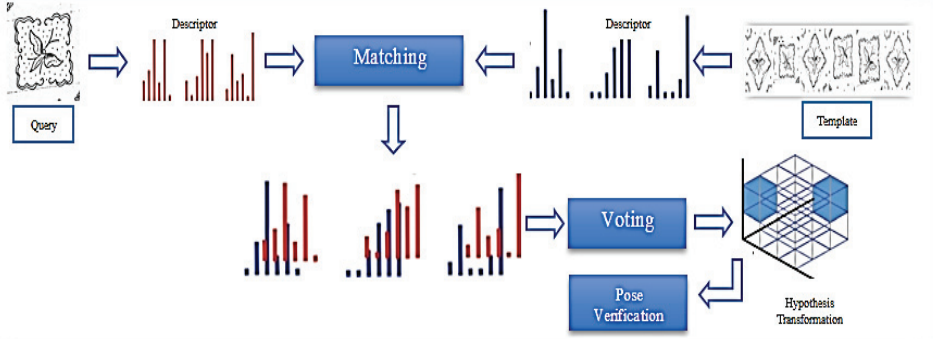
\includegraphics[width=1.0\linewidth]{sift-hough-voting-method}
		\caption{SIFT with hough voting method for Batik classification}
		\label{fig_sift_hough_voting_method}
    \end{figure}

\end{frame}

\begin{frame}{\cite{lowe2004distinctive}}

	\begin{figure}
        \centering
        \begin{minipage}{.5\textwidth}
            \centering
            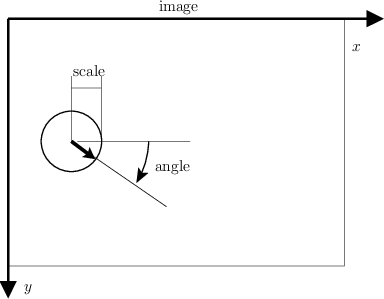
\includegraphics[width=.9\linewidth]{sift-keypoint}
            \caption{SIFT Keypoint}
            \label{fig_keypoint}
        \end{minipage}%
        \begin{minipage}{.5\textwidth}
            \centering
            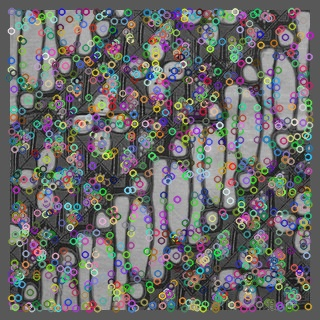
\includegraphics[width=.8\linewidth]{batik-parang-keypoints}
            \caption{SIFT Keypoints in Batik Parang}
            \label{fig_batik_parang_keypoints}
        \end{minipage}
    \end{figure}

\end{frame}

\begin{frame}{\cite{lowe2004distinctive}}

	\textbf{Distinctive image features from scale-invariant keypoints (2004)}
	
	{\small Lowe, David G}
	
	\begin{itemize}[<+->]
		
		\item SIFT keypoint is an \textbf{point of interest} in image obtained by detecting extrema of Difference of Gaussian (DoG) pyramid
		
		\item A keypoint has 4 parameters: center \textbf{coordinates} x and y, \textbf{scale} and its \textbf{orientation} (an angle expressed in radians) (Figure \ref{fig_keypoint})
		
		\item An image has \textbf{multiple keypoints} (Figure \ref{fig_batik_parang_keypoints})
		
		\item A keypoint descriptor is is a 3-dimensional (\textbf{128-elements sparse array}) spatial \textbf{histogram of the image gradients} characterizing a SIFT keypoint
		
	\end{itemize}

\end{frame}

\begin{frame}{\cite{lowe2004distinctive}}
	
	\begin{figure}
        \centering
        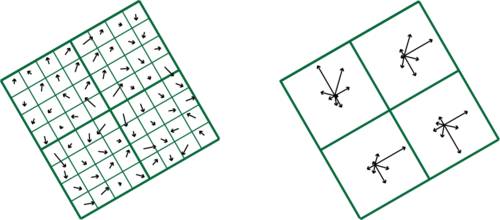
\includegraphics[width=1.0\linewidth]{sift-descriptor-1}
        \caption{SIFT descriptor}
        \label{fig_sift_descriptor_1}
    \end{figure}

\end{frame}

\begin{frame}{\cite{azhar2015batik}}

	\textbf{Batik Image Classification Using SIFT Feature Extraction, Bag of Features and Support Vector Machine (2015)}
	
	{\small Azhar, Ryfial and Tuwohingide, Desmin and Kamudi, Dasrit and Suciati, Nanik}
	
	\begin{itemize}[<+->]
		
		\item Classification using \textbf{support vector machine (SVM)} fed by \textbf{bag of words (BOF)} features extracted using \textbf{SIFT} descriptors
		
		\item SIFT descriptors were clustered using \textbf{k-means vector quantization} algorithm to build vocabularies for BOF
		
		\item Similar to \citep{nurhaida2015automatic}, SIFT descriptors are \textbf{not used directly} in matching
		
		\item \textbf{Very good} average accuracy of \textbf{97.67\%} for normal images, \textbf{95.47\%} for rotated images and \textbf{79\%} for scaled images
		
	\end{itemize}
	
\end{frame}

\begin{frame}{\cite{azhar2015batik}}
	\begin{figure}
		\centering
		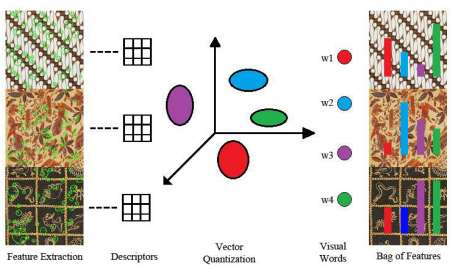
\includegraphics[width=1.0\linewidth]{sift-bag-of-words}
		\caption{SIFT for building bag of words visual vocabularies}
		\label{fig_sift_bag_of_words}
    \end{figure}
\end{frame}

\begin{frame}{\cite{willy2013evaluation}}

	\textbf{Evaluation of SIFT and SURF features in the songket recognition (2013)}
	
	{\small Willy, Dominikus and Noviyanto, Ary and Arymurthy, Aniati Murni}
	
	\begin{itemize}[<+->]
		
		\item Proved that \textbf{SURF were faster than SIFT} for Songket classification but had less accuracy
		
		\item Unlike \cite{moertini2005algorithms} and \cite{azhar2015batik} \textbf{SIFT and SURF features were directly} used to compute the matching scores
		
		\item Matching scores are calculated by (1) the number of \textbf{matched keypoints} and (2) the \textbf{average total distance of the n-nearest keypoints}
		
		\item Accuracy with SIFT features was \textbf{92-100\%} and \textbf{65-97\%} with SURF. 
		
	\end{itemize}
	
\end{frame}

\begin{frame}{\cite{willy2013evaluation} (continued)}

	\textbf{Evaluation of SIFT and SURF features in the songket recognition (2013)}
	
	{\small Willy, Dominikus and Noviyanto, Ary and Arymurthy, Aniati Murni}
	
	\begin{itemize}[<+->]
		
		\item With SURF features, the \textbf{accuracy dropped} quite significant if salt and pepper noises were added while SIFT was more stable. 
		
		\item Not paying much attention to \textbf{transformation variance} unlike \cite{azhar2015batik} and \cite{nurhaida2015automatic}
		
	\end{itemize}
	
\end{frame}


\begin{frame}{\cite{willy2013evaluation}}
	\begin{figure}
		\centering
		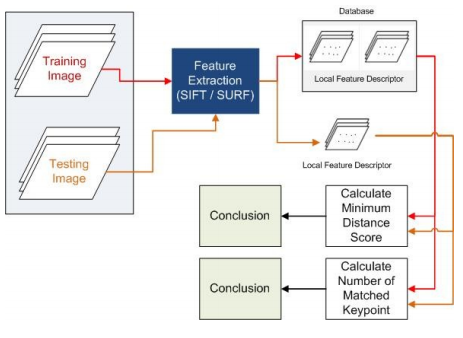
\includegraphics[width=.8\linewidth]{songket-sift-vs-surf-methodology}
		\caption{SIFT vs SURF method for Songket classification}
		\label{fig_songket_sift_vs_surf_methodology}
    \end{figure}
\end{frame}

\begin{frame}{\cite{lecun2015deep}}

	\textbf{Deep learning (2015)}
	
	{\small LeCun, Yann and Bengio, Yoshua and Hinton, Geoffrey}
	
	\begin{itemize}[<+->]
		
		\item Deep learning is a \textbf{multilayer representation learning} in artificial neural network
		
		\item Representation learning is a method in machine learning to \textbf{automatically extract/learn representation} (features) from raw data
		
		\item Basic deep learning architectures: convolutional neural network (ConvNet), deep belief network (DBN), autoencoder (AE) and recurrent neural network (RNN)
		
		\item Deep architectures can \textbf{extract transformation-variant features} (eg ConvNet for object detection)
		
%		\item Motivations 
%		\begin{enumerate}
%			\item New techniques (eg. pretraining \& dropout) and activation functions (eg. ReLU)
%			\item Big data 			
%			\item Fast hardware (GPU)		
%		\end{enumerate}
		
	\end{itemize}
	
\end{frame}

\begin{frame}{\cite{menzata2014sistem}}

	\textbf{Sistem perolehan citra berbasis konten dan klasifikasi citra batik dengan convolutional stacked autoencoder (2014)}
	
	{\small Menzata, Remmy Augusta}
	
	\begin{itemize}[<+->]
		
		\item Batik classification using \textbf{convolutional stacked autoencoder}
		
		\item Using convolutional transformations to \textbf{reduce the input nodes} of stacked autoencoder
		
		\item Achieved \textbf{81,73\%} accuracy (trained using small patches). When noises were added its accuracy dropped to \textbf{49\%} for gaussian noises, \textbf{61\%} for rotations, \textbf{70\%} for scalings and \textbf{75\%} for illumination noises. Less accurate than \cite{azhar2015batik} and \cite{nurhaida2015automatic}
		
		\item While \cite{fischer2014descriptor} showed that \textbf{ConvNet outperformed SIFT} 
		
	\end{itemize}
	
\end{frame}

\section{Future Works}

\begin{frame}{Future Works}
	
	\begin{itemize}[<+->]
	
		\item \textbf{Deep learning} architecture on Batik classification may give better result that current approaches as suggested by \cite{fischer2014descriptor}
		
		\item As mentioned in \cite{menzata2014sistem} suggestion, usage of \textbf{other deep architectures} than Convolutional Stacked Autoencoder such as Convulutional Neural Network (ConvNet) may improve result
		
		\item Consider \textbf{replacing SoftMax} layer with other algorithm such as Naive Bayes Classifier (NBC) or Support Vector Machine (SVM).
		
		\item \textbf{Transfer learning} model from another training session such as from popular VGG-16 by \cite{simonyan2014very}
	
	\end{itemize}
	
\end{frame}


\section{Research Proposal}

\begin{frame}{Research Proposal}

	\centering {\Large Batik classification using convolutional neural network (convnet) and transfer learning}
	
	\begin{itemize}
		\item Using dataset from \cite{menzata2014sistem}
		\item Experimenting with ImageNet model from \cite{simonyan2014very}
		\item Compare method with direct SIFT descriptor matching from \cite{willy2013evaluation}
	\end{itemize}

\end{frame}

\begin{frame}[allowframebreaks]{References}
  \bibliography{proposal}
  %\bibliographystyle{abbrv}
  \bibliographystyle{plainnat}
\end{frame}

\begin{frame}[standout]
  Thank you
\end{frame}


%\begin{frame}{Lists}
%  \begin{columns}[T,onlytextwidth]
%    \column{0.33\textwidth}
%      Items
%      \begin{itemize}
%        \item Milk \item Eggs \item Potatos
%      \end{itemize}
%
%    \column{0.33\textwidth}
%      Enumerations
%      \begin{enumerate}
%        \item First, \item Second and \item Last.
%      \end{enumerate}
%
%    \column{0.33\textwidth}
%      Descriptions
%      \begin{description}
%        \item[PowerPoint] Meeh. \item[Beamer] Yeeeha.
%      \end{description}
%  \end{columns}
%\end{frame}

%\begin{frame}{Animation}
%  \begin{itemize}[<+- | alert@+>]
%    \item \alert<4>{This is\only<4>{ really} important}
%    \item Now this
%    \item And now this
%  \end{itemize}
%\end{frame}


\end{document}
